\documentclass[11pt]{article}

\usepackage[utf8]{inputenc}
\usepackage[ngerman]{babel}
\usepackage{csquotes}

\usepackage{fullpage}
\usepackage{setspace}
\usepackage{parskip}
\usepackage{titlesec}
\usepackage{mathptmx}

\usepackage{graphicx}
\usepackage[section]{placeins}
\usepackage[justification=centering]{caption}
\usepackage{wrapfig}

\PassOptionsToPackage{
style=apa,
doi=false,
isbn=false,
eprint=false
}{biblatex}
\usepackage[backend=biber]{biblatex}
\addbibresource{ws1819_skribbl.bib}

\PassOptionsToPackage{hyphens}{url}

\makeatletter

\renewenvironment{abstract}
{{\bfseries\noindent{\abstractname}\par\nobreak}\footnotesize}
{\bigskip}

\renewenvironment{quote}
  {\begin{tabular}{|p{13cm}}}
  {\end{tabular}}

\titlespacing{\section}{0pt}{*3}{*1}
\titlespacing{\subsection}{0pt}{*2}{*0.5}
\titlespacing{\subsubsection}{0pt}{*1.5}{0pt}

\usepackage{authblk}

\usepackage[colorlinks = false]{hyperref}

\begin{document}

\begin{titlepage}
   \begin{center}
       \vspace*{1cm}

       \Huge
       Skribbl.AI Projektdokumentation (IQ vs. KI)
       \vspace{2.0cm}

       
\includegraphics[width=0.4\textwidth]{images/htw_logo.jpg}

       \vspace{1.5cm}
       \LARGE

       Josefine Sophie Busch, Malin Dulkies, Rachel Escueta, Tim-Niklas Heise, Ninoslav Kjireski, Anastasia Litvina, Anh Quang Vu-Tuyen

       \vfill

       Projektarbeit \\
       Prof. Dr. Klaus Jung\\
       Wintersemester 2018/2019\\

       \vspace{0.8cm}

       Hochschule für Technik und Wirtschaft\\
       Berlin\\

   \end{center}
\end{titlepage}

\pagebreak
\tableofcontents
\pagebreak
\listoftables
\listoffigures
\pagebreak

\section{Einleitung}
\subsection{Leitfaden}
\begin{wrapfigure}{R}{0.3\textwidth}
\centering
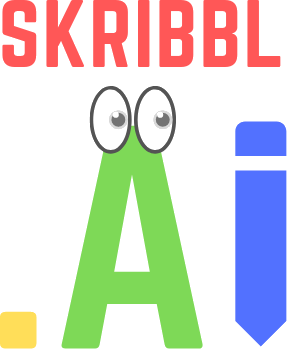
\includegraphics[width=0.25\textwidth]{images/skribbl_logo.png}
\caption{\label{fig:skribblLogo}Skribbl.AI Logo}
\end{wrapfigure}
Die Idee begann mit IQ gegen KI. Mit dem Einfall, was würde eigentlich passieren, wenn eine künstliche Intelligenz ein von einem Menschen gemaltes Bild  erkennen sollte? Neuronale Netzwerke erbringen beeindruckende Leistungen bei der Erkennung fotorealistischer Aufnahmen. Sie helfen sogar Pathologen bei der Erkennung von Krebszellen \parencite{ElizabethDougherty2018}. Was also würde also passieren, wenn wir eine künstliche Intelligenz mit den Kritzeleien einer Student*in konfrontieren?

 (Was ist das Projekt, wie ist es zustande gekommen, was ist das Ziel)
 \ref{fig:skribblLogo}

\subsection{Aufbau des Projektes}
    (Wir haben uns für agile, Scrum usw. entschieden)    1.2.1. Trello, Slack

\section{Grundlagen}
\subsection{Design}
2.1 Design( - Findung)(Hier kommt rein wie wir von AI vs KI zu Skribbl.AI gekommen sind)
Mobile First
Accessibility
Orientiert an SketchR
\subsection{Frontend}
\subsection{Neuronales Netzwerk}
\subsubsection{Dataset}
\section{Anforderungen}
Genauere Productvision, Detailierter
\section{Umsetzung, Implementierung, Ausarbeitung}
\section{Spielbeschreibung, Ziel}
\section{Bewertung}
vgl. Anforderungen mit Ergebnis

\printbibliography
\end{document}
